\section{Introduction}

Artificial Intelligence (AI) continues to reshape global industries, with Generative AI (GenAI) standing out as one of the most influential recent developments. GenAI models, such as large language models (LLMs) and diffusion architectures, have driven widespread adoption and significant investment, particularly in the technology sector. Yet, for retail investors, the tools available to access this growth remain largely generic and inaccessible, both in terms of domain focus and interpretability.

Private equity and venture capital investments in GenAI startups are becoming larger and more targeted as investor strategies evolve with the technology. Funding in GenAI exceeded \$56 billion in 2024, nearly double the \$29 billion recorded in 2023 \citep{spglobal2025}.

As shown in Figure~\ref{fig:genai-investment} below, while the number of funding rounds declined in 2024, the overall deal value surged. This suggests a consolidation of capital into larger, infrastructure-oriented bets, aligning with investor confidence in scalable GenAI deployments. These trends highlight the need for tools that help investors evaluate publicly listed companies best positioned to benefit from this structural shift.

\begin{figure}[h]
    \centering
    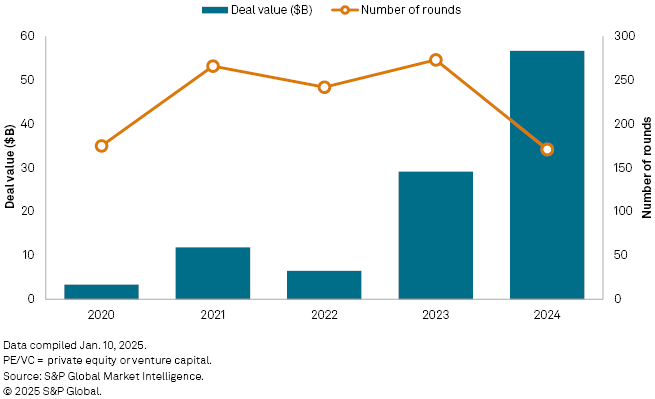
\includegraphics[width=0.5\textwidth]{assets/investGenAI.png}
    \caption{\small PE/VC investments in GenAI, 2020–2024. Source: S\&P Global Market Intelligence \citep{spglobal2025}.}
    \label{fig:genai-investment}
\end{figure}

This project responds to that gap by proposing the \textbf{GenAI Advisor}, a system that delivers explainable stock recommendations specifically for companies driving or enabling the GenAI revolution. Based on the \textit{Financial Advisor Bot} template, the system is designed for non-technical users, providing accessible, transparent investment signals that go beyond traditional model outputs.

\subsection{Concept}

The GenAI Advisor is conceived as a personalised financial guidance tool for individual investors interested in the GenAI sector. It provides interpretable recommendations, whether to buy, hold, or sell specific stocks, alongside human-readable explanations for these decisions. Unlike traditional investment tools that obscure decision logic behind opaque algorithms or technical jargon, this system foregrounds explainability and domain relevance.

The intended users of this system are individual retail investors interested in emerging technology themes but lacking the technical background to interpret raw financial signals or operate sophisticated trading tools. These users are typically non-specialists with limited exposure to algorithmic finance or machine learning models. For this group, the GenAI Advisor offers an accessible tool to support their decisions, that reduces complexity while preserving analytical rigour. It is also suitable for students, educators, or early-stage investors exploring explainable AI in financial contexts.

At its core, the GenAI Advisor is built on the belief that financial tools should be not only accurate but also comprehensible. This is particularly important in thematic investing, where users are drawn not only by quantitative performance but by interest in specific technological trends. In this context, the system acts as a digital intermediary between complex market signals and users' intuitive understanding, offering advice that is grounded and traceable, with a clearly scoped set of companies.

The conceptual novelty lies in its hybrid orientation; it combines evidence-driven financial analysis with a commitment to interpretability. The Advisor does not aim to outperform the market through high-frequency trading (HFT) or proprietary forecasting. Instead, it prioritises accessibility, domain focus, and trustworthiness, delivering insights users can understand and apply in their decision-making. In doing so, it invites users into the analytical process rather than substituting for it.

Furthermore, the GenAI Advisor embraces thematic integrity by carefully curating its stock universe. It avoids general-purpose technology firms in favour of those with demonstrable involvement in the GenAI ecosystem, whether through infrastructure, tooling, model development, or deployment. The rationale for company inclusion and exclusion is detailed in the project scope (Section~\ref{sec:scope}). This conceptual grounding ensures that recommendations are not only technically derived but also strategically aligned with the user's thematic intent.

\subsection{Motivation}

The motivation for this project is both technical and user-oriented. GenAI represents an emerging thematic investment opportunity that remains underserved by existing tools. Simultaneously, there is increasing demand for transparent and accessible AI systems tailored to the needs of retail investors in the financial domain.

Traditional robo-advisors, such as Nutmeg and Moneyfarm, provide automated portfolio allocation but are domain-agnostic and opaque in how decisions are made. While open-source trading bots like Freqtrade offer flexibility, they require technical expertise and lack natural language interfaces. StockGPT \citep{mai2024stockgpt} demonstrates the potential of generative models in stock prediction, while recent work on XAI-integrated forecasting \citep{marey2024xai} highlights the importance of trust and interpretability in financial AI systems.

By combining simple rule-based logic with predictive models and natural language explanations, the GenAI Advisor aims to deliver recommendations that are not only accurate but also intelligible. A local LLM serves as an interpretive layer rather than a decision engine, ensuring that outputs remain grounded in logic and statistical inference, while still being comprehensible to the user.

Beyond usability, the project contributes to responsible AI by ensuring data privacy and reproducibility. No personal or sensitive data is collected, and all sources are public. The LLM is hosted locally to avoid transmitting user inputs externally. The system is explicitly intended for educational and demonstrative use, and includes appropriate disclaimers to distinguish it from regulated financial services.

\subsection{Scope}
\label{sec:scope}

The GenAI Advisor focuses on a curated set of publicly traded companies whose business models are materially driven by Generative AI. The portfolio includes firms across three categories: (1) software developers and strategic investors (e.g., Microsoft, Alphabet, Meta, Amazon); (2) hardware providers (e.g., Nvidia, AMD, Intel, Marvell); and (3) infrastructure suppliers (e.g., TSMC, SK hynix, Broadcom, Arista Networks). These companies were selected for their direct contributions to GenAI model development, deployment, or enablement.

To maintain thematic focus and ensure data availability, the system excludes private companies, indirect holdings, and general technology firms lacking core GenAI offerings (e.g., Apple, Netflix). Chinese firms (e.g., Alibaba, Tencent, Baidu) are also excluded due to market access limitations \citep{usdoc2022exportcontrols} and restricted financial transparency due to the Variable Interest Entity (VIE) structure of the BATX (Baidu, Alibaba, Tencent, and Xiaomi) stocks \citep{chen2021vie}.

This scope ensures the system operates within a clearly bounded, analytically defensible domain. It enhances the relevance of recommendations by aligning them with user intent and facilitates reproducible evaluation by focusing on transparent and publicly accessible data.